\documentclass[../Hovedrapport.tex]{subfiles}
\begin{document}
%-----------------------------------------------------------------------------------------------------------------
\chapter{Forsøgsresultater}
    \label{chap:Forsøg}
        \vspace{-30pt}
%-----------------------------------------------------------------------------------------------------------------
Konstruktionen af aggregater såsom køleskabe består ofte af en iterativ proces, hvor idéer og beregninger bliver ført ud i livet gennem prototyper. Disse tidlige udgaver af et produkt er sjældent fejlfrie, men kan i stedet belyse hvilke dele af systemet, der skal korrigeres inden den næste prototype bliver konstrueret. I netop tilfældet med et køleskab er det essentielt, at fordamperen har den rette kuldeydelse, således anlægget opfylder sit primære formål om at køle mad- og drikkevarer til en ønsket temperatur. Som led i at opnå den ønskede kuldeydelse skal systemets tryk og temperaturer undersøges samt varmetilførslen fra indsatte varmelegemer og omgivelserne under realistiske forhold.   

Dette afsnit tager afsæt i forsøgsrapporten udarbejdet i forbindelse med dette projekt. For dybere gennemgang af forsøgene henvises der til denne rapport. 

\section{Forsøgbeskrivelse (N.J. \& J.K.)}

Denne rapport består af fire forsøg, som har til formål at belyse fordamperens kuldeydelse sammenlignet med den teoretisk beregnede værdi samt køleskabets evne til at opretholde en konstant temperatur under forskellige scenarier med belastninger. Det første forsøg vil således fungere som en kontrol af beregningerne, mens de tre øvrige forsøg tager afsæt i situationer, som et køleskab i en bar jævnligt vil blive udsat for. 

\subsubsection*{Forsøg 1}
Indledningsvist vil forsøg 1 afdække, hvorledes fordamperberegningerne er i overensstemmelse med den kuldeydelse, som bestemmes under forsøget. Denne vil blive bestemt på baggrund af de målte lufttemperaturer før og efter fordamperen i en situation, hvor køleskabet belastes maksimalt ved åbning af køleskabsdøren. 

\subsubsection*{Forsøg 2}
Det andet forsøg tager udgangspunkt i, at det er afgørende, at et køleskab er i stand til at opretholde den ønskede temperatur, når varmere legemer indsættes. Tilmed skal de mad- eller drikkevarer, som allerede befinder sig i køleskabet, ikke undergå en temperaturstigning, som medfører at kvaliteten af varerne falder jf. afsnit \ref{sec:kravspec}. I forsøget vil to vandflasker befinde sig i køleskabet ved \SI{4}{\celsius}, hvorefter 38 flasker ved stuetemperatur indsættes i køleskabet. Temperaturforløbet for de to oprindelige vandflasker vil blive dokumenteret for at klarlægge de øvrige flaskers indvirkning. 

\subsubsection*{Forsøg 3}
Tredje forsøg fokuserer på, hvordan et køleskab placeret i en bar vil blive påvirket af, at døren hyppigt åbnes, når barens kunder skal betjenes. Dette vil medføre en varmetilførsel fra de ydre omgivelser ind i køleskabet og til dets indhold. Forsøget har derfor til formål at dokumentere temperaturforløbet for luften i køleskabet, samt de nedkølede vandflasker, over 30 minutter, hvor køleskabet åbnes 24 gange á 30 sekunders varighed. 

\subsubsection*{Forsøg 4}
Slutteligt vil det fjerde forsøg tage afsæt i scenariet, hvor en betydelig mængde drikkevarer, ved stuetemperatur $21\si{\celsius}$, indsættes i køleskabet, med henblik på at få disse nedkølet så hurtigt som muligt. I den forbindelse vil temperaturforløbet for vandflasker og køleskabsluften blive målt, hvorved varmetilførslen fra flaskerne efterfølgende kan bestemmes. 

\section{Resultater (N.J. \& J.K.)}
\subsubsection*{Forsøg 1}
Den maksimale kuldeydelse målt i forsøg 1 er \si{624} $\pm$ \SI{16,0}{W}, når køleskabet belastes maksimalt muligt ved at have døren hertil åben uafbrudt. Kuldeydelsen ved en lufttemperatur på \SI{10}{\celsius} i køleskabet er desuden blevet bestemt til \si{510} $\pm$ \SI{15,3}{W}, hvilket ikke afviger signifikant fra den teoretisk beregnede værdi på \SI{454}{W}, der er udregnet med samme fremgangsmåden som i afsnit \ref{sec:dim_fordamper} dog ved en lufttemperatur på \SI{10}{\celsius}. Det ses desuden, at trykket og dermed også fordampningstemperaturen er en smule højere end de beregnede \SI{2,17}{bar}, hvor den mindste er blevet målt til \SI{2,31}{} $\pm$ \SI{0,07}{bar}. Dette indikerer, at fordamperen kan optage tilstrækkeligt med varme og muligvis er en smule større end først antaget. Varmeveksleren i forsøget har bølgede lameller, hvilket der ikke er taget højde for i beregningerne. Dette giver en mere turbulent strømning og derved en bedre varmeovergang. 

\subsubsection*{Forsøg 2}
I forsøg 2 er de to kolde vandflaskers temperaturer blevet logget, og det ses herved, at temperaturen for den øverste og nederste vandflaske, når en maksimalværdi på henholdsvis \si{6,7} $\pm$ \SI{1,4}{\celsius} og \si{6,5}$\pm$ \SI{1,4}{\celsius} inden temperaturerne begynder at falde ned til \SI{4}{\celsius} igen. Således har de 38 flasker en indvirkning på de to kolde vandflasker, hvilket resulterer i en kortvarig temperaturstigning. På baggrund af grafer med temperaturen for køleskabsluften og vandflaskerne er det samtidig blevet belyst i forsøget, at hvis kompressoren er for længe om at starte igen under reguleringen, vil dette hurtigt have en indvirkning på temperaturerne i vandflaskerne, som kortvarigt stiger inden kompressoren igen tændes.   

\subsubsection*{Forsøg 3}
Ved det tredje forsøg er temperaturerne for de to vandflasker blevet bestemt til henholdsvis \si{4,8}$\pm$ \SI{1,4}{\celsius} for den nederste flaske og \si{6,1}$\pm$ \SI{1,4}{\celsius} for den øverste. Disse temperaturer er bestemt efter en halv times belastning ved gentagende åbninger af køleskabsdøren. Temperaturforløbet for de to vandflasker samt køleskabsluften fremgår af figur \ref{fig:temp_forsoeg3} nedenfor. Flaske 1 placeret på den øverste hylde har en orange graf, mens Flaske 2 på den nederste hylde er blå. Den gennemsnitlige lufttemperatur i køleskabet har en grå graf. 

\begin{figure}[H] % (alternativt [H])
	\centering
	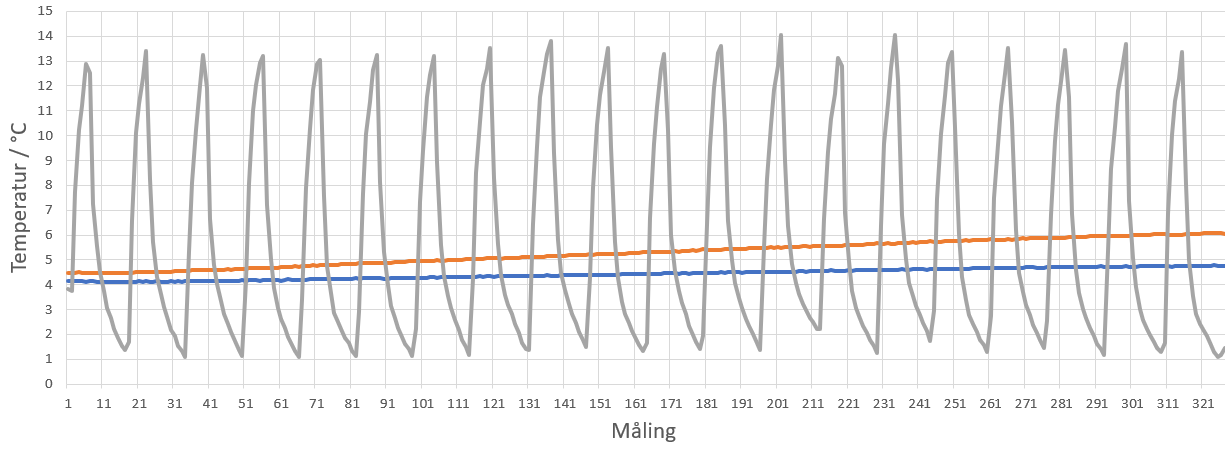
\includegraphics[width=1.0\textwidth]{Billeder/Temperaturforloeb.PNG}
	\caption{\textit{Temperaturforløb for vandflasker og køleskabsluft i Forsøg 3.}}
	\label{fig:temp_forsoeg3}
\end{figure}

Det fremgår desuden af øvrige grafer i Forsøg 3, at kompressoren er i stand til at få køleskabets lufttemperatur tilbage til den ønskede i løbet af 1 minut. Varmestrømmen fra de ydre omgivelser er slutteligt blevet bestemt til \si{348} $\pm$ \SI{98,4}{W} ved åbning af døren, hvilket dog afviger betydeligt fra den teoretiske værdi på \SI{1950}{W}. Den teoretiske værdi er beregnet med fremgangsmåden beskrevet i afsnit \ref{sec:aabning_af_dor} blot ved en udvendig lufttemperatur på \SI{21}{\celsius}. De nærmere beregninger fremgår af appendiks \ref{sec:doeraabning_21C}. Afvigelsen kan bl.a. skyldes, at volumenstrømmen i praksis ikke er lige så stor, da fordamperen, hylderne og vandflaskerne er med til at hindre luftstrømmen rundt i køleskabet. Derudover tager formlen for den teoretiske varmestrøm ikke højde for størrelsen af køleskabets volumen, hvor der i dette tilfælde hurtigt vil ske en udskiftning af luften. Dette betyder, at varmestrømmen $\Phi_{\text{dør}}$ kun har denne størrelse momentant.

\subsubsection*{Forsøg 4}
I det fjerde og sidste forsøg er den maksimale varmestrøm fra de 40 vandflasker blevet bestemt til \si{175} $\pm$ \SI{0,025}{W} på baggrund af de målte temperaturer i vandflaskerne under nedkølingen. Dette afviger fra den teoretisk beregnede i ligning \ref{eq:flaske_samlet} på \SI{306}{W}. Afvigelsen skyldes, at temperaturdifferensen under forsøget er på \SI{11}{K} og dermed er mindre end den anvendte i beregningerne. Indsættes denne differens fra forsøget i den teoretiske beregning fås dog en varmestrøm på \SI{198}{W}, hvilket er betydeligt tættere på. De nærmere udregninger fremgår af appendiks \ref{sec:varmeafgivelse_ved_21grader}. Slutteligt er varmegennemgangstallet for flaskevæggen blevet bestemt til \si{13,4} $\pm$ \SI{0,002}{\frac{W}{m^2 \cdot K}} i dette forsøg, mens den teoretisk beregnede værdi er \SI{15,9}{\frac{W}{m^2 \cdot K}}. Den forholdsvis lille afvigelse mellem det målte og beregnede varmegennemgangstal skyldes formodentlig, at varmeovergangstallene er baseret på erfaringsmæssige værdier. Den minimale usikkerhed for de forsøgsbestemte værdier skyldes, at resultaterne er beregnet ud fra en regressionsligning over flaskernes temperaturforløb, som antages at være ideel. 

Tabel \ref{tab:vent_maalt_para} samler de mest væsentlige parametre med deres teoretiske værdi samt den værdi målt og beregnet i praksis:
\begin{table}[H]
\centering
\begin{tabular}{|c|c|c|c|} \hline \rowcolor[gray]{.7}
\multicolumn{4}{c}{\textbf{Beregnede og målte parametre}} \\ \hline \rowcolor[gray]{.8}
Parameter           & Forventet    & Målt $\pm$ Usikkerhed & Afv. fra forventet \\ \hline
$\Phi_0$            & \SI{454}{W}  & \SI{510} $\pm$ \SI{15,3}{W} & \SI{12,3}{\%} \\ \hline
$\Phi_{\text{dør}}$ & \SI{1950}{W} & \SI{348} $\pm$ \SI{98,4}{W} & \SI{82,1}{\%} \\ \hline
$\Phi_{flasker}$    & \SI{198}{W} & \SI{175} $\pm$ \SI{0,025}{W} & \SI{11,6}{\%} \\ \hline
$U_{flasker}$       & \SI{15,9}{\frac{W}{m^2 \cdot K}} & \SI{13,4} $\pm$ \SI{0,002}{\frac{W}{m^2 \cdot K}} & \SI{15,7}{\%} \\ \hline
$p_{R,f}$           & \SI{2,17}{bar} & \SI{2,31} $\pm$ \SI{0,07}{bar} & \SI{6,45}{\%} \\ \hline
\end{tabular}
\caption{\textit{Oversigt over forventede og beregnede parametre}.}
\label{tab:vent_maalt_para}
\end{table}

\end{document}